\documentclass[12pt]{article}
\usepackage{geometry}
\geometry{a4paper, margin=1in}
\usepackage{graphicx}
\usepackage{titlesec}
\usepackage{xcolor}
\usepackage{hyperref}
\usepackage{fancyhdr}
\usepackage{enumitem}

% Formatting
\titleformat{\section}{\large\bfseries}{\thesection.}{0.5em}{}
\pagestyle{fancy}
\setlength{\headheight}{15pt}
\fancyhf{}
\rhead{EE175A/B – Weekly Progress Report}
\lhead{Battery Management and Communication System}
\rfoot{Page \thepage}

\begin{document}

\begin{center}
    {\Large \textbf{Weekly Progress Report (WPR)}} \\[6pt]
    {\large \textbf{Battery Management and Communication System (BMS)}} \\[2pt]
    \rule{0.8\textwidth}{0.5pt} \\[6pt]
\end{center}

\noindent
\textbf{Team:} Kaushik Vada, Christian Kim, Connor Stewart, Nick Poon \\[3pt]
\textbf{Course:} EE175B – Senior Design II \\
\textbf{Instructor:} Prof. Roman Chomko \\
\textbf{Week:}(\textit{Jan 26 – Feb 1, 2026}) \\[8pt]

\vspace{1em}

\section{Work Completed This Week}
\begin{itemize}[leftmargin=1cm]
    \item Completed 3D printing of the BMS enclosure and improved CAD design optimizations.
    \item Iterated through multiple CAD versions and physical 3D prints to address dimensional inconsistencies.
    \item Refined tolerances to ensure seamless assembly of all components.
    \item Optimized the enclosure layout to be compact while maintaining full functionality.
    \item Commenced firmware development by analyzing the E-Load and BMS schematics and successfully initializing their respective pins to ensure proper communication and control.
\end{itemize}

\vspace{1em}

\section{Challenges Encountered}
\begin{itemize}[leftmargin=1cm]
    \item Achieving precise tolerances in 3D printed parts to fix measurement inconsistencies.
    \item Balancing spatial optimization (compactness) with necessary functionality.
\end{itemize}

\vspace{1em}

\section{Work Plan for Next Week}
\begin{itemize}[leftmargin=1cm]
    \item Begin working on the FMS (Fault Management System) logic and diagrams.
\end{itemize}

\vspace{1em}

\section{Appendix A – System Block Diagram}
\begin{center}
    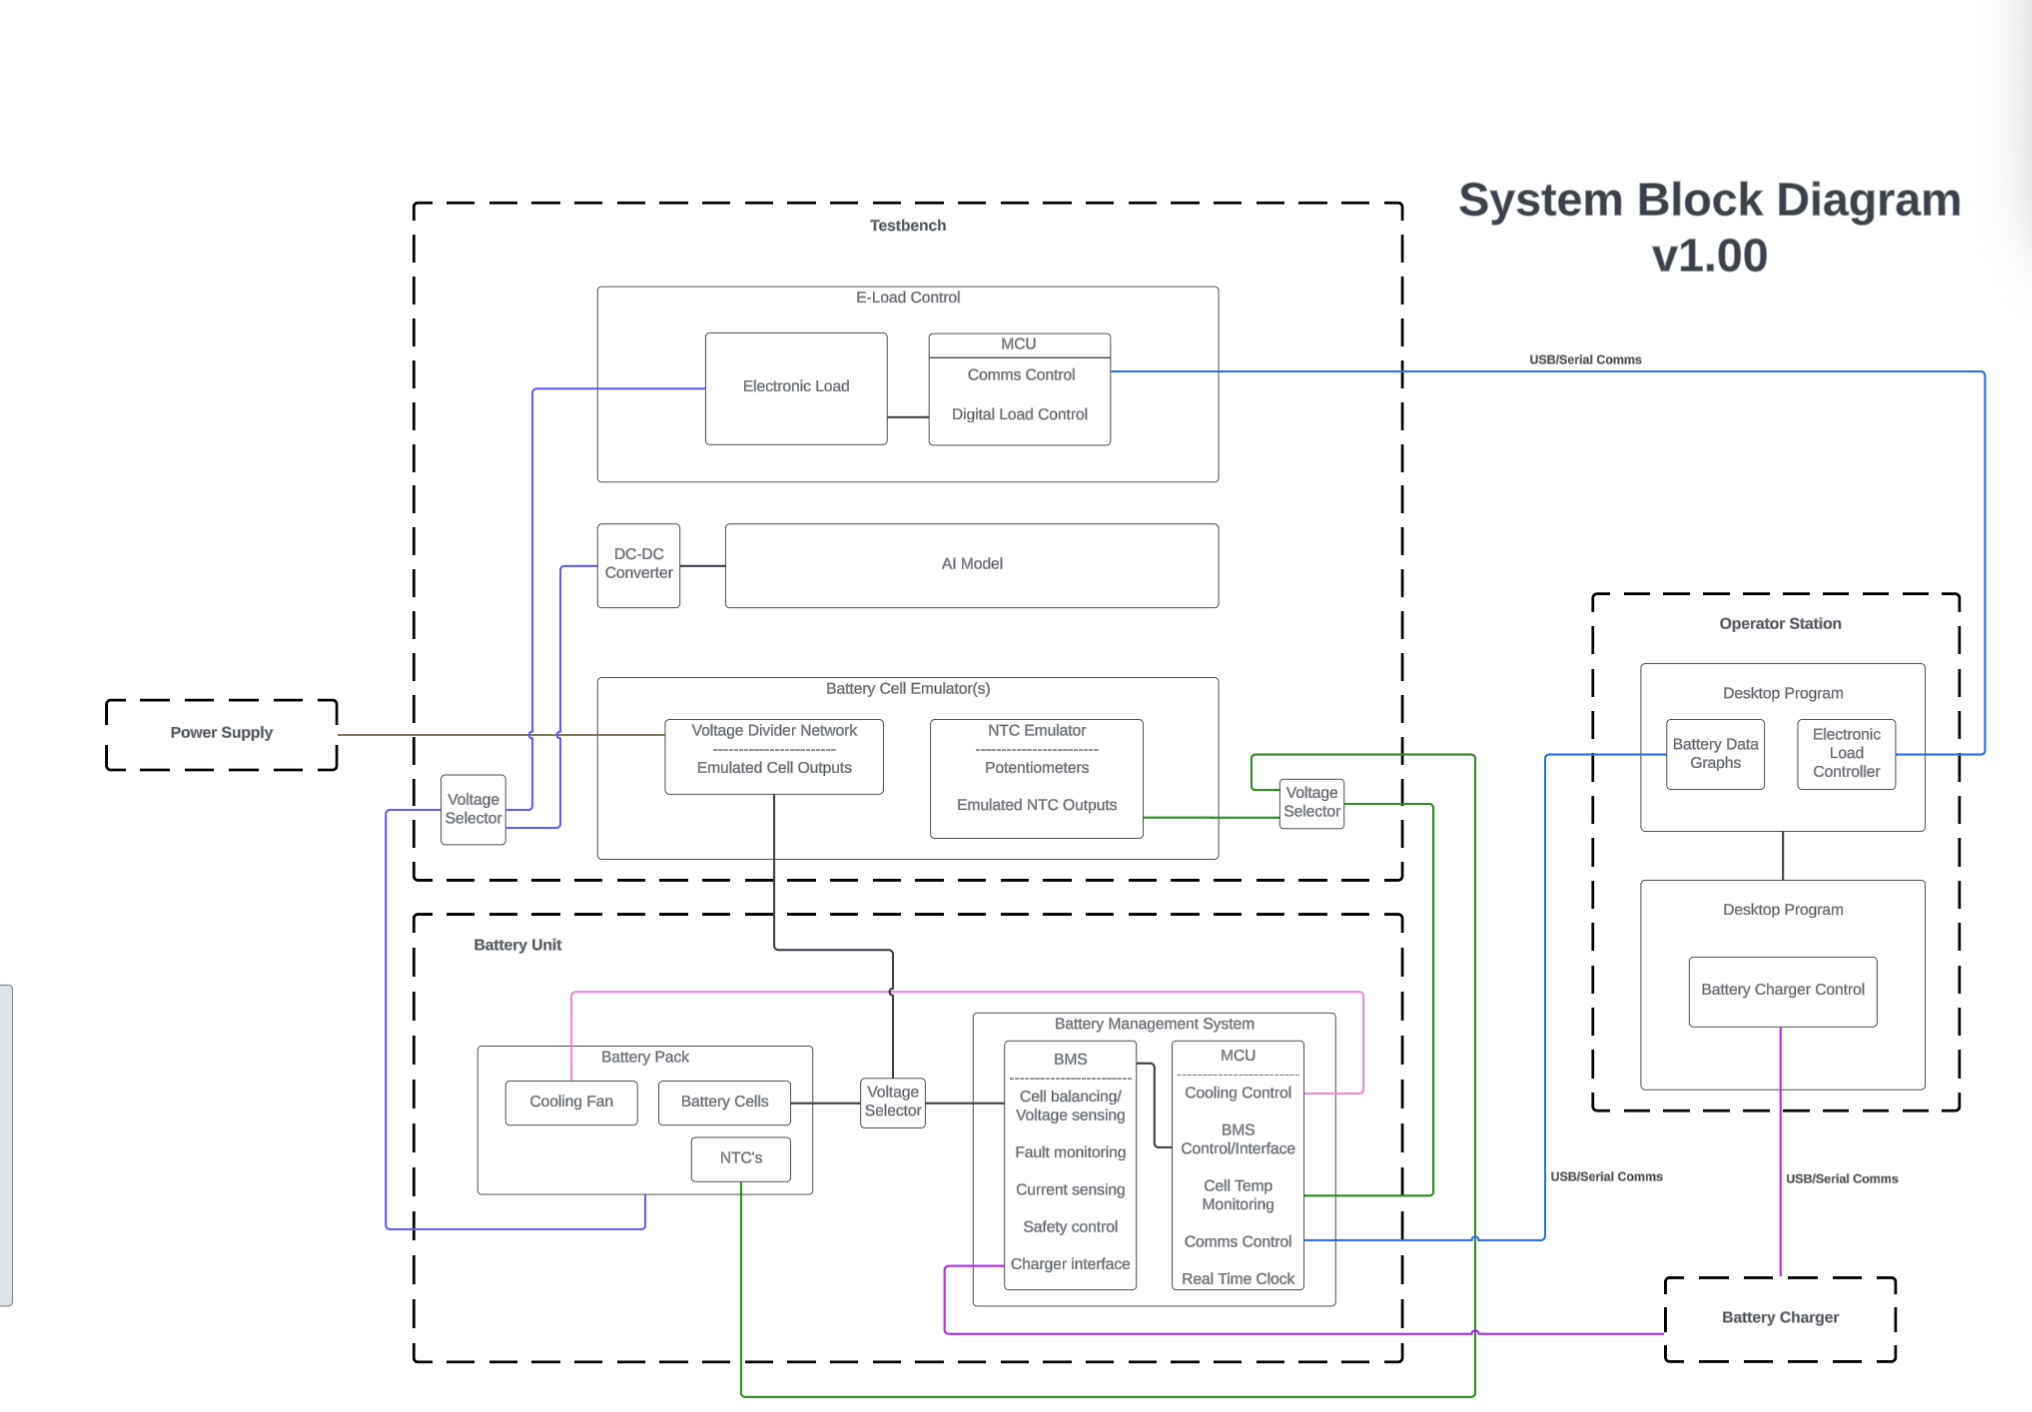
\includegraphics[width=0.95\textwidth]{bms_block_diagram.png} [Figure 1]
\end{center}
\noindent
\textit{Figure A1:} Updated System Block Diagram showing battery domain, isolation components, STM32 communication, and host interface (Source: EE175 Project Report).

\vspace{1em}

\section{Appendix B – Enclosure Visualization}
\begin{center}
    \includegraphics[width=0.95\textwidth]{BMS_enclosure.png} [Figure 2]
\end{center}
\noindent
\textit{Figure B1:} 3D rendering of BMS enclosure with semi-transparent lid, showing airflow, fan, USB-C port, and internal component placement.

\vspace{1em}

\section{Appendix C – Battery Pack Implementation}
\begin{center}
    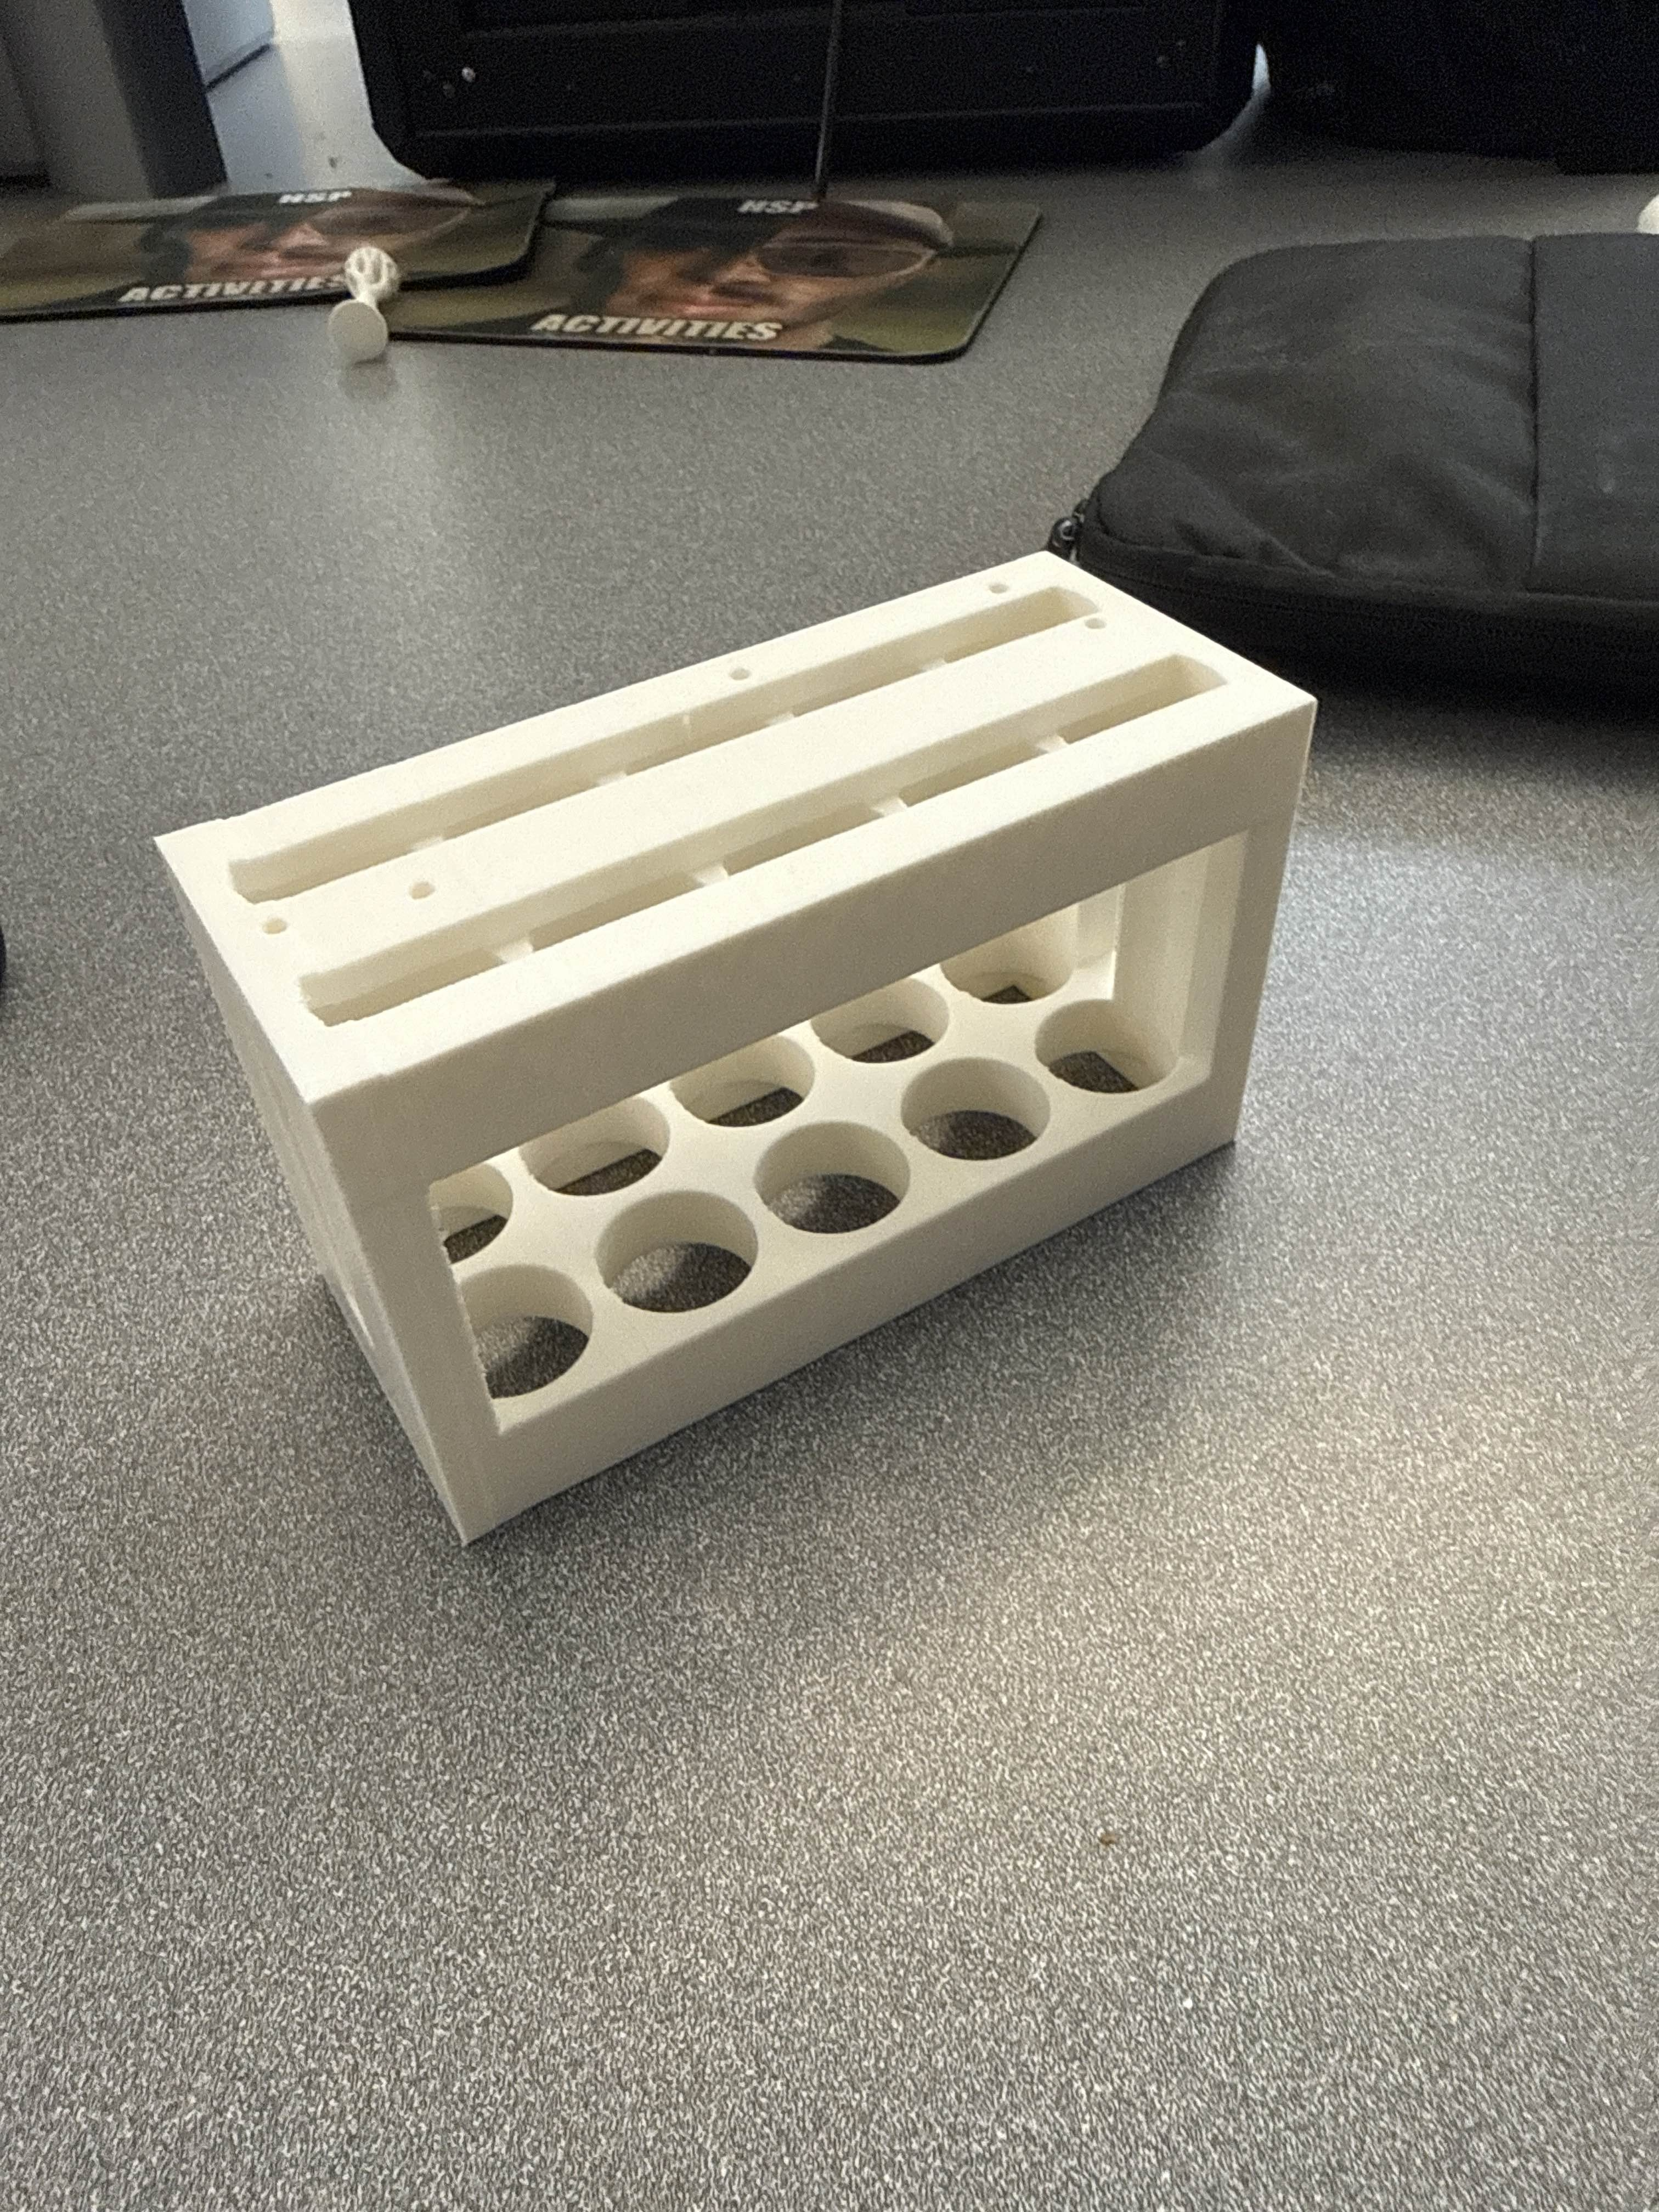
\includegraphics[width=0.95\textwidth]{Battery_Pack.png} [Figure 3]
\end{center}
\noindent
\textit{Figure C1:} Battery pack assembly showing cell arrangement and integration with the BMS unit.

\vspace{1em}

\end{document}